\chapter{Adaptive Sampling Theory}
\label{ch:chapter3}
In this chapter, we investigate the theory of Adaptive sampling and different Markov processes, transfer operators and their dominant spectrum.The results stated here were originally published in paper \cite{Adstrategies2018} including the figures in this chapter.

intor, upper limit conlucsion


\chapter{Adaptive Sampling Comparison}
\label{ch:chapter32}

The results stated here were originally published in paper\cite{Adstrategies2018} including the figures in this chapter.

\RED{until here ok}
Ever increasing demand for high data rate wireless transmissions with high spectral efficiency leads to utilization of communication systems with multiple transmit and receive antennas. Excellent quality of service represented with near-channel capacity error-rate performance can be achieved with iterative receiver structure composed of inner soft detection and outer soft-input soft-output decoding. Emerging wireless standards such as:~Wireless Local Area Network (W-LAN), Worldwide Interoperability for Microwave Access (WiMAX), $3^{rd}$ Generation Partnership Project Long Term Evolution (3GPP-LTE), etc are being constantly revised to provide higher data rates and better error-rate performance. Iterative receivers based on inner soft detection and outer decoding are promising solutions.

In this thesis, we propose to address issues of designing efficient physical layer receiver structure targeting its use in emerging wireless systems, including both downlink and uplink scenarios. It is our goal to develop performance-efficient wireless receiver with implementable hardware cost while achieving data throughputs in the order of hundreds MBits/sec. 

\section{x}
\label{sec:x3}
Excellent error-rate performance in MIMO environment are made possible by employing sophisticated algorithms such as maximum \emph{a posteriori}~(MAP) detection techniques and outer channel decoding that provides error-correction in the presence of multiple access interference, burst channel fading, channel multi-paths, additive receiver noise, etc. An approximation of impractically complex optimal joint detection/decoding is achieved by iteratively improving the \emph{a posteriori} probabilities (APPs) of transmitted coded bits between inner soft detection and outer decoding


\section{\label{sec:intro2}Introduction}

Molecular dynamics (MD) simulations have become indispensable for gaining
insight into molecular systems at high spatial and temporal resolutions.
However, a key limitation for MD with accurate all-atom force-fields remains
the computational demand for simulating processes with long timescales. In
particular, biologically relevant processes, such as protein folding and
conformational changes, typically require simulation time in excess of
milliseconds, while atomic-resolution MD trajectories can currently reach
timescales on the order of microseconds on standard computational resources. 

In the last decade, significant efforts have been devoted to alleviate the MD
timescale problem.
In general, such efforts can be divided into three broad categories. In the
first category, the use of different computational resources has allowed the
simulation of longer timescales, either by cumulating trajectories from
massively-distributed computing \cite{DistComp-Shirts2000, DistComp-Buch2010}
or by the design of special-purpose hardware \cite{shaw2014anton}.
The second class of methods can be characterized by their ability to
accelerate the occurrence of rare events in simulation, thereby reducing the 
actual computational time needed to observe biophysically relevant
processes in practice. Examples in this class include accelerated MD
\cite{hamelberg2004accelerated}, replica-exchange MD \cite{sugita1999replica}
and metadynamics \cite{laio2008metadynamics}. While these methods improve the
efficiency of sampling and can be used for thermodynamics studies, they 
alter the system's Hamiltonian, and can not be directly used to extract kinetic
information from the simulation. Path reweighting
methods \cite{pathreweight1, pathreweight2, pathreweight3, pathreweight4}
have been recently proposed to recover the kinetic information
after altering the system's Hamiltonian.

The third class of methods can be grouped under the term \emph{adaptive
sampling} \cite{singhal2005error, bowman2010enhanced,
weber2011characterization, Fabritiis-2014, preto2014fast, doerr2016htmd,
AdaptivePELE-Lecina2017, EvolutionCoupling-Shamsi2017, FAST-Bowman-2015, 
Strategies-erros-reduce, plattner2017complete}. An analysis of the power and
limitation of such methods is the subject of this work. 

Instead of simulating long MD trajectories to observe rare events, adaptive sampling
methods take a ``divide and conquer'' approach and attempt to iteratively
combine many short MD simulations, distributing them in a way to 
escape from local free energy minima, and efficiently visit different regions of
the conformational space of the systems of interest.
At each iteration, all of the simulations that have been performed at that
point are pooled and analyzed. New simulations are then initialized by
using the information extracted from the analysis of the previous iterations.
The main idea of adaptive sampling is that, by periodically analyzing the
conformational space already explored, new simulations can be restarted 
in a way that may significantly enhance the probability of observing rare
events. The choice of the strategy chosen to restart the trajectories is crucial
to the success of the approach, and several different methods have been
proposed \cite{weber2011characterization, Fabritiis-2014,
AdaptivePELE-Lecina2017,preto2014fast, doerr2016htmd,roblitz2013fuzzy,
weexplore, WESTPA-Zwier2015}.
Recently, enhanced sampling in combination with adaptive sampling methods has
also been proposed~\cite{pathreweight5}.


The popularity of adaptive sampling methods is due to the significant advances in the
analysis of MD trajectories. In the last decade, different methods have been
put forward to extract essential information from high dimensional MD data to a
small number of reaction coordinates associated with the slow
collective processes in the system's dynamics \cite{rohrdanz2013discovering,
noe2017collective}. Such methods include Markov State Models (MSMs) \cite{prinz2011markov,
MSM-Pande-2018,bookmsm,masterequationsMSM,SCHUTTE1999146}, Diffusion Maps
\cite{Coifman7426, rohrdanz2011determination,Zheng2011, Boninsegna2015}, likelihood based approaches
\cite{peters2006obtaining}, cut-based free energy profiles
\cite{krivov2008diffusive}, or neural networks \cite{Mardt2018,wehmeyer2018time,
ribeiro2018reweighted}.  In particular, MSMs provide a good complement for
adaptive sampling as they are designed to handle many short trajectories and
do not require an equilibrium sampling to recover global thermodynamics and
kinetic properties (such as metastable states, free energy barriers, and
transitions between states), as long as the trajectories are in local
equilibrium.  

As mentioned above, different adaptive sampling methods can be characterized by how the
information extracted from previously explored space is used to
initiate new trajectories at each iteration.
Although the power of adaptive sampling has been demonstrated by successful
applications \cite{Wieczorek2016,Plattner20171005,Kohlhoff201415}, there is no general consensus as to how to
choose a particular method over another for a specific system. If the goal is
to simulate a rare event such as protein folding, does a method based on eigenvalues
outperform one based on counts? Could the same adaptive sampling method be then
used for general exploration of conformational space? Additionally, previous
studies \cite{preto2014fast,weber2011characterization,bowman2010enhanced,Fabritiis-2014} report efficiency gains with
adaptive sampling between a factor 2 and a factor of 10. What characteristics of the system of
interest can we use to predict that a particular adaptive sampling method will
provide a better efficiency gain?  Here we present a systematic study on a
number of model systems to address these questions.
In particular, we consider the efficiency of different adaptive sampling strategies for
two different goals on a number of model systems: to speedup the simulation
time needed to observe a specific rare event, such as the folding of a protein,
or to speedup the exploration of large regions of the conformational space of
the same protein.

In order to be able to benchmark and compare the results on different systems, we
use previously generated extensive MD trajectories \cite{lindorff2011} to
generate 8 discrete models for protein dynamics.
The results of this analysis reveal that different strategies are needed
for different goals. In particular, on-the-fly estimation of global
equilibrium properties from non-equilibrium data is very important to speedup
the folding of a protein, while the knowledge of equilibrium properties is not
needed if the goal is the exploration of large regions of the conformational
space (independently if folded or unfolded). This result suggests that
different strategies may need to
be combined in various stages of a specific application to both enhance the
occurrence of a rare event and appropriately sample the different metastable states.
Comparison of the results on different proteins
suggest that the speedup that can be achieved by adaptive sampling is larger
for slower processes, thus encouraging the application to more complex systems.


\section{\label{sec:methods}Methods}

%As mentioned above, adaptive sampling methods rely on two main ingredients: 1)
%A procedure to separate, at least locally, slowly mixing configurations from
%fast mixing ones, by using the partial information available from the space
%already sampled. This information can then be used to cluster together the fast
%mixing configurations and discretize the space into a set of N states; and 2)
%A strategy to restart the simulations from the any of the states already
%explored in order to maximize the probability of escaping to yet unexplored
%states.
\subsection{\label{sec:methods-dataset}Dataset of Simulations}

We used previously existing long all-atom MD trajectories
of 8 different small proteins\cite{lindorff2011}, obtained on the Anton supercomputer, to generate
discrete model systems, as discussed below. The dataset is summarized in Table
\ref{tab:dataset-summary} and contains proteins ranging from 10 to 80 residues,
with different topologies ($\alpha$-helices, $\beta$ sheets, or a mix of both),
simulated folding times ranging from $0.6$ to $49$ $\mu$s, and different timescale gaps between
the folding process and other competing slow processes.

\begin{table}[!ht]
\centering
\caption{Previously simulated proteins used to generate discrete models in this study}
\label{tab:dataset-summary}
%\begin{tabular}{ccccc}
\resizebox{\columnwidth}{!}{
\begin{tabular}{|c|c|c|c|c|c|}
\hline
Protein Name & PDB ID of Folded Structure & Size (\# residues) & Folding Time ($\mu$s) from \cite{lindorff2011}\\ 
\hline
Chignolin    & 2RVD                       & 10                 & 0.6                 \\
Trp-cage     & 2JOF                       & 20                 & 14                  \\
BBA          & 1FME                       & 28                 & 18                  \\
WW Domain    & 2F21                       & 35                 & 21                 \\
Protein B    & 1PRB                       & 47                 & 3.9                  \\
Homeodomain  & 2P6J                       & 52                 & 3.1                  \\
$\alpha$3D   & 2A3D                       & 73                 & 27                  \\
$\lambda$-repressor  & 1LMB               & 80                 & 49             \\ 
\hline            
\end{tabular}
}
\end{table}

\subsection{\label{sec:methods-msm}Construction of discrete protein models}

To emulated adaptive sampling, an MSM was generated for each protein from
the previously existing long all-atom MD trajectories, then synthetic
microstate trajectories are generated by sampling the MSM transition matrix.
An MSM models the system's dynamics by discretizing the explored
conformational space into a finite number of states, and estimating their
probability and the probability of transition between them \cite{prinz2011markov}.
The analysis is summarized by a transition matrix,
$T_{ij}$, that indicates the probability that the system transitions from state
$i$ to state $j$ within a chosen lag time $\tau$. The discretization of the
original conformational space into states (also called microstates) is usually
performed by clustering the configurations sampled by MD trajectories using
a distance metric that can separate slowly mixing configurations from rapidly
interconverting ones \cite{noe2016commute, Noe2015}.

We have used standard procedures to perform these steps. In particular, for
each protein, we used the Time-lagged Independent Component Analysis (TICA) 
\cite{TICA1-perez2013, TICA2-schwantes2013} combined with the commute map 
\cite{noe2016commute}, to reduce the dimensionality of the system. As an input
for TICA, each conformation was first featurized using all pairwise
inter-residue distances (between the two closest heavy-atoms) and all dihedral
angles along the protein chain.
For smaller systems, the reciprocals of the inter-residue distances were also
used as additional features. The Euclidean distance between the
lower-dimensional points in the commute map space provides a good measure to
obtain a kinetically meaningful state decomposition, and an associated MSM
\cite{noe2016commute}. All conformations were then
partitioned with k-means clustering into 1000 or 2000 microstates, depending on
the size of the protein. It was ensured that the slowest MSM eigenvector is the
folding-unfolding process and all microstates are connected by removing
disconnected microstates. Finally, the transition matrix for the MSM is
computed using maximum-likelihood estimation with a detailed balance
constraint. The lag time, $\tau$, for the MSM was chosen based on the
convergence of the implied timescales, and the Markovianity property of the MSM
was tested by using the Chapman-Kolmogorov test \cite{prinz2011markov}. All the
analysis was performed using the PyEMMA Python package \cite{scherer2015pyemma}
and the exact parameters for the construction of discrete protein models for
each protein are listed in the Supplementary material.

\subsection{\label{sec:level5}Simulating Trajectories using MSMs}

Adaptive sampling involves iteratively running many short MD trajectories, and
different adaptive sampling methods differ in how the new structures are chosen
to initialize the next round of MD trajectories. We can simulate the adaptive
sampling process of iteratively running an ensemble of $n$ MD trajectories 
using the transition matrix from an MSM as follows. 
Note that the restart strategies here are concerned with selecting states
visited among the discrete set of microstates in the MSM. 
In actual molecular dynamics simulations, continuous trajectories in a protein
configurational space are used instead of the synthetic trajectories generated here
by jumping between the different discrete states of an MSM in adaptive step 2.
Therefore, in actual simulations the analysis (adaptive step 3 below) involves also the
the discretization of all the available trajectories into a set of microstates.

\begin{figure}[!ht]
  \centering
  \includegraphics[width=0.5\textwidth]{figures/schema4.pdf}
  \caption{Adaptive sampling strategy schema}
  \label{fig:schema}
\end{figure}

\begin{itemize}
\item Adaptive step 1: Start with a randomly chosen unfolded state from the discrete set of microstates available for a given protein
\item Adaptive step 2: Generate $n$ independent discrete trajectories (of a fixed length) from the selected state(s)
using the probabilities from the MSM transition matrix 
\item Adaptive step 3: Analyze the ensemble of trajectories generated
\item Adaptive step 4: Select $n$  microstates among the ones visited so far from which to start the next round of trajectories 
\item Adaptive step 5: Repeat adaptive steps 2,3 and 4 or finish after a certain number of iterations

\end{itemize}

We denote the adaptive steps 3 and 4 together as the \emph{restart strategy} for an
adaptive sampling method. Figure~\ref{fig:schema} is a graphical representation
of the process. The different restart strategies that we use in this work are
described in detail in the following section. When using continuous trajectories from actual molecular dynamics simulations,
the analysis step 3 also includes the discretization of the continuous
trajectories into discrete trajectories (for instance, by means of TICA and MSM).
Thus, the restart strategy for adaptive sampling in actual molecular dynamics
simulations must also select a set of individual conformations or frames from the selected
microstates to initialize the next MD simulation. This can be done for example in
a uniformly random fashion within the microstate or by selecting a representative
conformation. 
The length of the trajectories in each iteration can be varied, but it needs to
be larger than the lag time used to generate the MSM.
Here we chose the length of each short MD trajectory the same as the lag time
$\tau$, that is, the analysis is performed after the discrete trajectories have
been propagated by one step of length $\tau$. 
At each iteration, for a given strategy, the $n$ restarting points for the new
trajectories are chosen independently of each other.

In order to study the speedup in folding, subsets of the discrete microstates for
each protein are denoted as folded and unfolded states. 
Using the PDB files from Table \ref{tab:dataset-summary}, the native contacts
are extracted for the folded structure of each protein. A native contact is
defined if the distance between the two closest heavy atoms in a pair of
residues is 4\r{A} or less. For each state in the MSM, we compute the median number of native
contacts over all the conformations mapped to the state. States above a threshold
value for the number of native contacts are assigned as a folded state. States
below a threshold value for the number of native contacts are assigned as an
unfolded state. The threshold values for individual proteins can be found in the Supplementary material. 

\subsection{\label{sec:restart-strategies}Restart Strategies for Adaptive Sampling}

For each protein model, we use the MSM analysis and adaptive sampling procedure detailed
above with different restart strategies. We use a number of popular
strategies that do not assume a priori knowledge of the system, such as the microstate counts, or strategies that assume some a
priori knowledge of the system, such as the number of native contacts. 

%Since MSMs are usually the central
%analysis of the trajectories, new restarting structures can also be chosen
%based on improving the quality of the final MSM \cite{singhal2005error,
%bowman2010enhanced}.

Here we describe all the restart strategies that we have used on all the
different protein models. Several of these strategies require to set the value
of some parameters, which are provided in the Supplementary material. 

\paragraph{MD} 
As a reference, we generate synthetic MD trajectories without any adaptive
choice of the restart points. No analysis is performed after each
iteration, and each trajectory is restarted from the same state where it
ended in the previous iteration. That is, the restart state chosen for
trajectory $n_i$ at iteration $t$ is simply the state of trajectory $n_i$ at
iteration $t-1$.

%As a reference the folding of the proteins with plain molecular dynamics (MD)
%simulation was simulated with discrete trajectories. This allows calculating
%the speedup of the adaptive sampling strategies compared to the plain MD
%simulation. By allowing 

\paragraph{Microstate Counts ($1/C$)}
One intuitive and popular restart strategy consists in choosing the restart
states based on how many times the previous trajectories have visited each state
in the conformational space
\cite{weber2011characterization, Fabritiis-2014, AdaptivePELE-Lecina2017}, in
order to favor less populated states.  In particular, a
given state $i$ is chosen as restart state with a probability inversely
proportional to the number of times it has been visited.

\RED{\emph{cmacro}}
\paragraph{Macrostate Counts ($1/C_M$)} 
Another count-based method that has been used in different applications clusters all the
visited microstates into fewer metastable macrostates on-the-fly. Usually, eigenvectors of
a matrix summarizing the sampling performed are used for the clustering
\cite{preto2014fast, doerr2016htmd}.  Here we use the transitions between all
the visited microstates to build an on-the-fly MSM, and the microstates are
clustered into macrostates using PCCA+ \cite{roblitz2013fuzzy}. 
%Any not fully connected microstates are treated as additional macrostates.
The restart state is then chosen with the following procedure. A macrostate
is first chosen with probability inversely proportional to the number of times
the macrostate has been visited. Then a microstate within the chosen macrostate
is chosen with probability inversely proportional to the number of times the
microstate has been visited. We have tested four variations of this strategy.
The first two variations (named $1/C_{M,1}^C$ and $1/C_{M,2}^C$) make use of the count
matrix $C_{ij}$ to directly estimate the on-the-fly MSM transition matrix. The count matrix
$C_{ij}$ contains the number of transitions that have been recorded in previous
iterations from state $i$ to state $j$. Every time a state is visited, the corresponding value
in the count matrix is incremented by one. This count matrix is normalized such
that each row sums to one and then used to estimate the on-the-fly MSM for the
adaptive sampling strategies.
The two variations differ as follows:
\begin{description}
\item[$1/C_{M,1}^C$]
PCCA+ is used to cluster the microstates into 30 macrostates.
\item[$1/C_{M,2}^C$]
The number of macrostates generated by PCCA+ is based on the number of
significant timescales using a 50\% kinetic content cutoff \cite{noe2016commute}.
\end{description}

The next two variations (named $1/C_{M,1}^K$ and $1/C_{M,2}^K$) are used to
estimate the effect of using non-equilibrium trajectories for the adaptive sampling
strategies. Since in most adaptive sampling methods many relatively short
trajectories are used, the non-equilibrium sampling can introduce errors in the
analysis of these trajectories.
Recently, the Koopman reweighting method
\cite{koopmanold, koopman2,koopman3,koopman4, wu2017variational, Nueske2017} has been
introduced to correct for the non-equilibrium effects in estimating global
equilibrium properties and can significantly reduce this error. In order to
evaluate the effect of the non-equilibrium sampling error in the performance of
the adaptive sampling strategy, we assume that the use of Koopman reweighting
in the analysis of MD trajectories can provide an accurate estimate of the
equilibrium transition probabilities between any pair of explored microstates.
Thus, in the synthetic trajectories used here, at each iteration, we estimate
an on-the-fly Koopman-corrected MSM by using the true transition probability
between the explored microstates (properly renormalized) and discarding any
transition to unexplored states.  Two more variants are studied by applying this correction to the previous two: 
\begin{description}
\item[$1/C_{M,1}^K$]
PCCA+ is used to cluster the microstates into 30 macrostates, on the Koopman-corrected MSM
\item[$1/C_{M,2}^K$]
The number of macrostates generated by PCCA+ on the Koopman-corrected MSM is
based on the number of significant timescales using a 50\% kinetic content
cutoff \cite{noe2016commute}.
\end{description}

\paragraph{$Q_{f}$ - Native Contacts}
If additional information is available on the system of interest, it can also be used to
guide the sampling. For instance, it has been proposed
\cite{EvolutionCoupling-Shamsi2017} to select restarting structures for
adaptive sampling based on the number of contacts likely made in the folded
states based on an evolutionary coupling analysis. Alternatively, the FAST
method \cite{FAST-Bowman-2015} was proposed as a way to exploit a priori
information, such as the distance to a target structure.  Here, we
consider the case where the folded structure is known, and the number of native
contacts can be used as a reaction coordinate for the folding
process. Out of the states already visited by the simulation, states with a
higher median number of native contacts are chosen with higher probability than
states with a lower number of native contacts. The probability of choosing a
visited state $i$ is proportional to $exp( - k * | Q_i - Q_{max} | )$, where
$Q_i$ is the number of native contacts in state $i$, $Q_{max}$ is the total number of
native contacts, and $k$ is a parameter of the strategy (see Supplementary material).

\RED{remove supplementary }
\paragraph{$Q_{f,nn}$ - Native and Non-native contacts} 
A variation of the previous strategy is to use two reaction coordinates in the
case when the folded structure is known, keeping track of the number of both
native and non-native contacts that are formed during the simulation. For each
state in the MSM, we compute the median number
of native and non-native contacts over all conformations mapped to each state.
Out of the states already visited by the simulation, states with a higher
number of native contacts have a higher probability of being chosen as
restarting points, as in the $Q_{f}$ strategy described above. Additionally,
states with a lower number of non-native contacts are chosen with a higher
probability than states with a higher number of non-native contacts. The
probability of choosing a visited state $i$ is proportional to $exp(-d_i)$,
where $d_i = \sqrt{k_1^2 * (Q_i - Q_{max})^2  + k_2^2 * N_i^2}$. $Q_i$
is the number of native contacts in state $i$, $Q_{max}$ is the total number of
native contacts, $N_i$ is the number of
non-native contacts in state $i$, and $k_1, k_2$ are parameters of the
strategy. One can think of $d_i$ as a distance to the folded state in
native/non-native contact space (scaled by $k_1$ and $k_2$). The two parameters
$k_1$ and $k_2$ were optimized by a parameter sweep (see Supplementary material). 
In real simulations such an optimization of the parameters is not
possible, but we perform it here to estimate the upper bound for the speed up.

\paragraph{$p_{esc}$ - Optimal strategy for exploration}
We also test a strategy that is not feasible in practice but offers a baseline
comparison as a theoretically optimal one. This strategy is built by using knowledge
of the full transition matrix of the system, that is not a priori known in real
applications (it is usually the goal of the sampling).
For each visited microstate $i$, we
compute the probability to transition to any microstate not yet explored using
the true transition matrix:
%
$$p_{esc}[i]=\sum_{j \in unexplored}T[i, j]$$
%
The state with the highest $p_{esc}$ value is chosen as the restart state. As stated above,
this strategy is impossible to implement in practice for real protein
simulations, but it is as a useful benchmark for comparing adaptive sampling
strategies that aim to explore conformational space.

\paragraph{$t_{opt}$ - Optimal strategy to speedup slow processes (protein folding)} 
We also test another theoretically optimal strategy given perfect knowledge of the
system dynamics as well as knowledge of the folded states. In a way that is
similar to the definition of mean first passage time \cite{mfptbook},
for each state $i$ in the MSM, we compute a value $t_{opt}[i]$ which 
estimates the minimal time to reach the folded state.
We first define that for each folded state $f$, $t_{opt}[f] = 0$. Then we
iteratively solve the following recurrence relation for each state $i$ outside the folded region:
%
$$t_{opt}[i]=1+\sum_{j \in states}T[i,j]min(t_{opt}[i],t_{opt}[j])$$
%
The equation is solved iteratively until the relative change in $t_{opt}$ drops
below a cutoff. We then use it to define a benchmark restart strategy, by
selecting the restart state among the ones explored that has the lowest
$t_{opt}$ value, representing the state that is the closest to the folded
state. Note again that this strategy is impossible to implement in
practice, but still is a useful benchmark for adaptive sampling strategies.
With the $t_{opt}$ benchmark the maximum achievable speedup with adaptive
sampling for the folding of a protein can be evaluated.

\section{\label{sec:results}Results}

In order to quantify the performance of different adaptive sampling strategies,
we considered two broad measures of efficiency. The first measure is the time
it takes for a strategy to simulate a rare event, in terms of steps of synthetic
trajectories. For the dataset used here, the rare event of interest is the
folding process and, for all proteins considered, the slowest timescale (or
rarest event) is the folding timescale. For each strategy, the average time measured
for a given strategy to reach the folded state starting from an unfolded state
is compared with the corresponding time in the absence of adaptive sampling
(that is, for the MD strategy described above). The second measure is one
that focuses on the exploration of the configurational space instead of a single
rare event. For any given strategy, we measure the time needed to explore 95\%
of the states used to build the MSM and compare it with the corresponding MD time.
For each protein, we evaluate these two measures for each of the adaptive
sampling strategies described above. Each strategy is evaluated by using a different
number of parallel trajectories $n$, ranging from 1 to 5000. 
The results reported
are averaged over 100 independent runs per protein and per number of parallel
trajectories.

\subsection{\label{sec:time-fold}Time to fold}

\begin{figure}[t!]
  %%\centering
  \begin{subfigure}[t]{0.5\textwidth}
    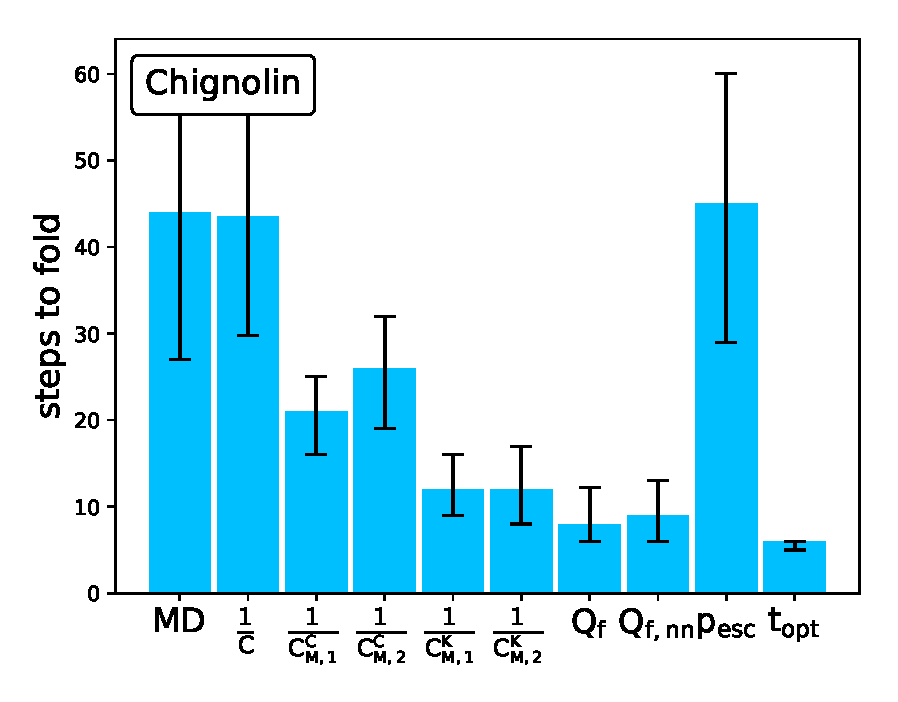
\includegraphics[width=0.9\textwidth]{figures/CLN025_7_steps10000_nparallel100_fold.eps}
    %%\caption{Chignolin}    
  \end{subfigure}
  \begin{subfigure}[t]{0.5\textwidth}
    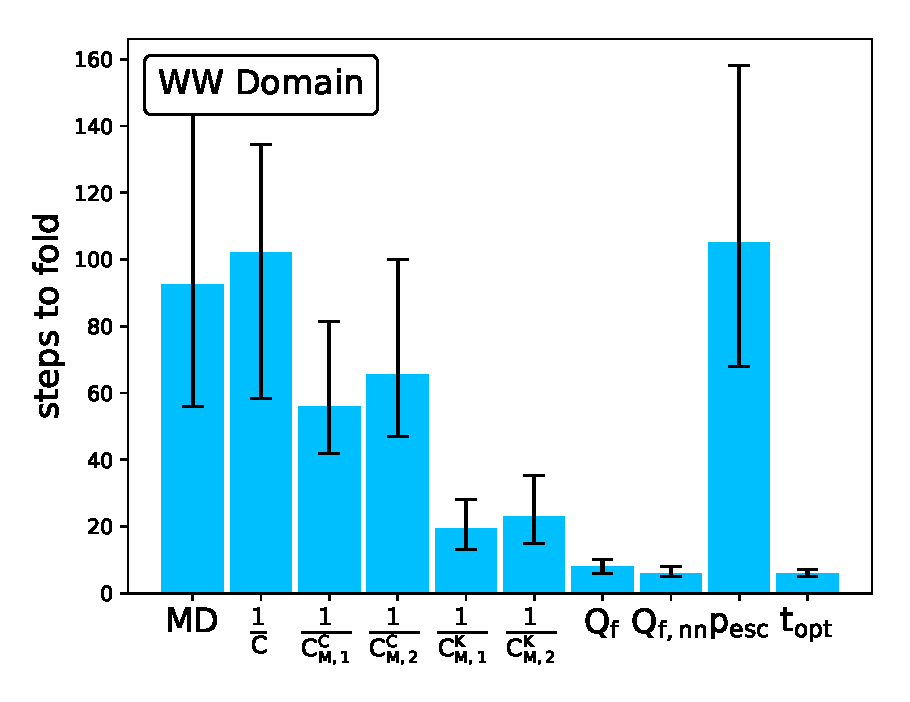
\includegraphics[width=0.9\textwidth]{figures/GTT_7_steps10000_nparallel100_fold.eps}
    %%\caption{WW Domain}    
  \end{subfigure}
  \begin{subfigure}[t]{0.5\textwidth}
    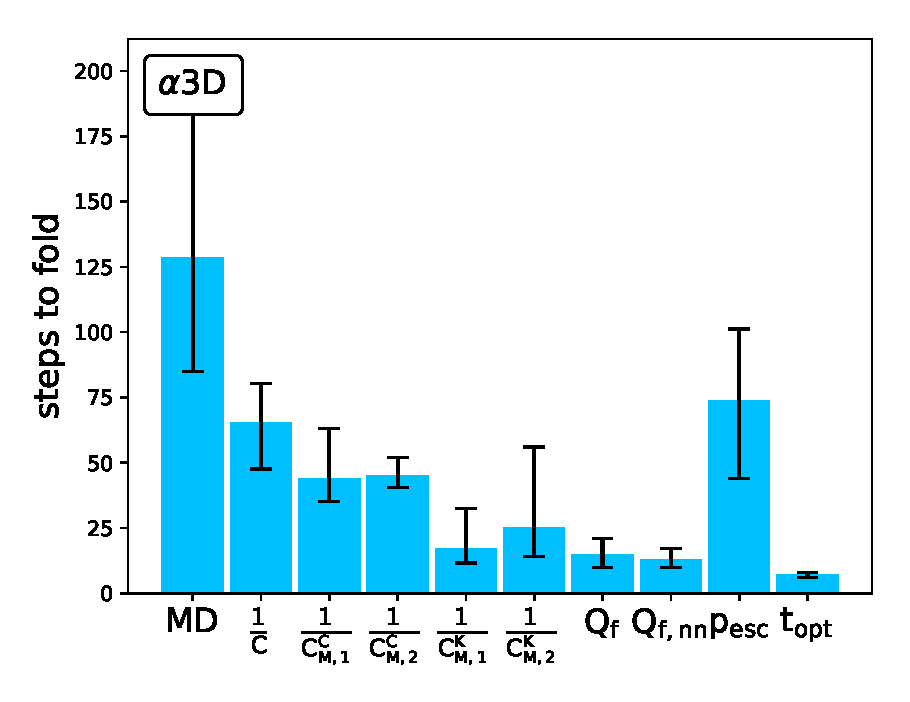
\includegraphics[width=0.9\textwidth]{figures/A3D_7_steps10000_nparallel100_fold.eps}
    %%\caption{$\lambda$-repressor}    
  \end{subfigure}
  \caption{Comparison of the number of steps of synthetic trajectories required
  to fold for the different adaptive sampling strategies for three different
  proteins using 100 parallel trajectories. The 20\% and 80\% percentiles are
  shown as the error bars. The results of the t-test between MD and the
  individual strategies for the different proteins are reported in the Supplementary material.}
  \label{fig:Time_fold}
\end{figure}

Figure~\ref{fig:Time_fold} shows the average folding time for each of the
strategies for three different proteins using 100 parallel trajectories. First, we note that the
popular microstate-based $1/C$ strategy does not always appear to speedup the
folding time, while the macrostate-based methods do show significant
improvement over MD. 
Interestingly, the benchmark strategy designed to maximize the probability to
visit unexplored regions of the configurational space  ($p_{esc}$, defined
above) does not significantly speedup the sampling of the folding rare event.
Both $1/C$ and $p_{esc}$ are strategies designed for general exploration and
not specifically for rare event sampling, and it is not surprising that these
strategies do not perform well in accelerating folding events.
Instead, the macrostate-based methods appear to successfully introduce a
sampling bias toward states that are along the direction of the slowest
timescale, as manifested in the significant speedup with respect to simple MD.
These results are consistent over the set of model proteins studied.

Within the macrostate-based methods, the correction for non-equilibrium that
can be achieved by Koopman reweighting ($1/C_M^K$) appears to further improve
the sampling of the rare folding event over using a simple uncorrected count
matrix ($1/C_M^C$) in the on-the-fly MSM definition. The correction for
non-equilibrium allows a more accurate estimation of the leading eigenvector of
the true transition matrix over using the raw, on-the-fly count matrix. Thus,
the resulting macrostates are more kinetically relevant. We also observe that
the results obtained when the number of macrostates is defined by the kinetic
content ($1/C_{M, 2}$) do not differ significantly from what is obtained when a constant number
of macrostates is used ($1/C_{M, 1}$). In some instances, it appears that using
kinetic content slightly hurts the performance of the adaptive sampling, which
may be due to inaccurate estimation of the timescales in the early stages
of the simulation.

Finally, we observe that incorporating a reaction coordinate, such as the
number of native contacts in the strategies does indeed significantly improve
the sampling of rare events. The improvement is, in fact, close to the
theoretical maximum that is estimated by $t_{opt}$. We also observe that the
addition of the number of non-native contacts as a second reaction coordinate
does not always improve the performance of the algorithm. In particular, this
is true for the smallest of the protein model considered (Chignolin), the
kinetics of which does not exhibit any additional slow processes besides
folding (see Fig.~\ref{fig:Time_fold}). For all the other protein models, the
introduction of a second reaction coordinate very marginally improves the
sampling of the folding process.
These patterns are consistent across all the proteins and across the number of
parallel trajectories used. The plots for all proteins (in addition to
Fig.~\ref{fig:Time_fold}) can be found in the Supplementary material.


\subsection{\label{sec:time-explore}Time to explore 95\% of states}

\begin{figure}[!hbt]
  %%\centering
  \begin{subfigure}[t]{0.5\textwidth}
    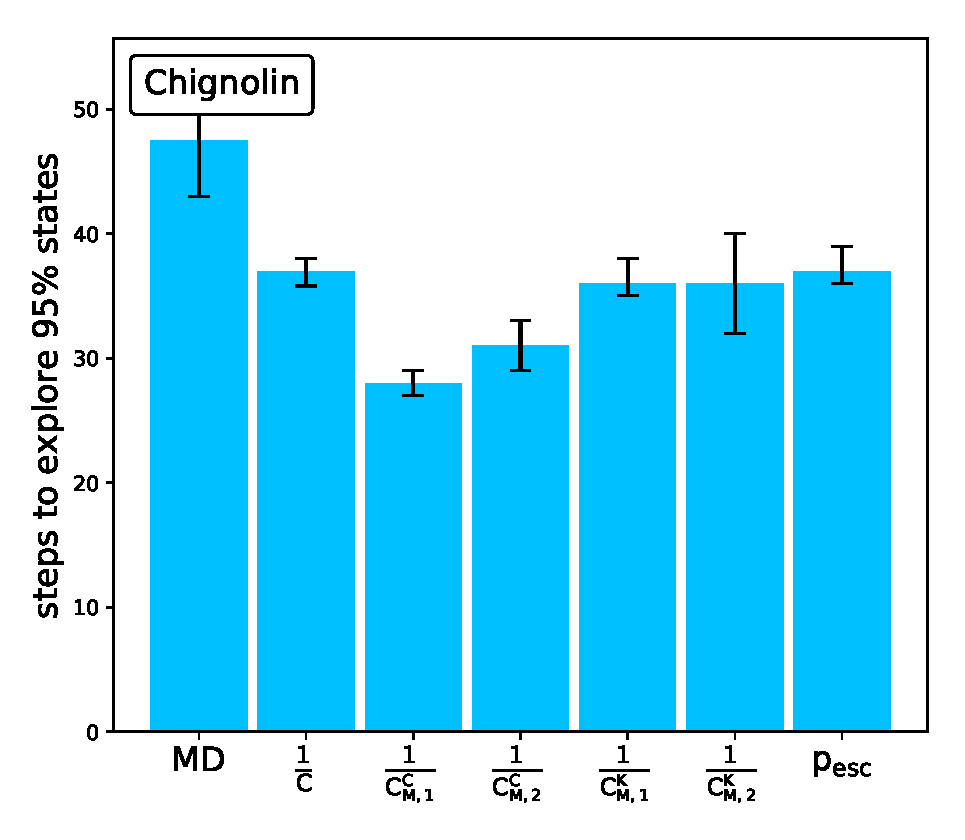
\includegraphics[width=0.9\textwidth]{figures/CLN025_7_steps10000_nparallel100_explore.eps}
    %%\caption{Chignolin}   
    %%[width=\textwidth] 
  \end{subfigure}
  \begin{subfigure}[t]{0.5\textwidth}
    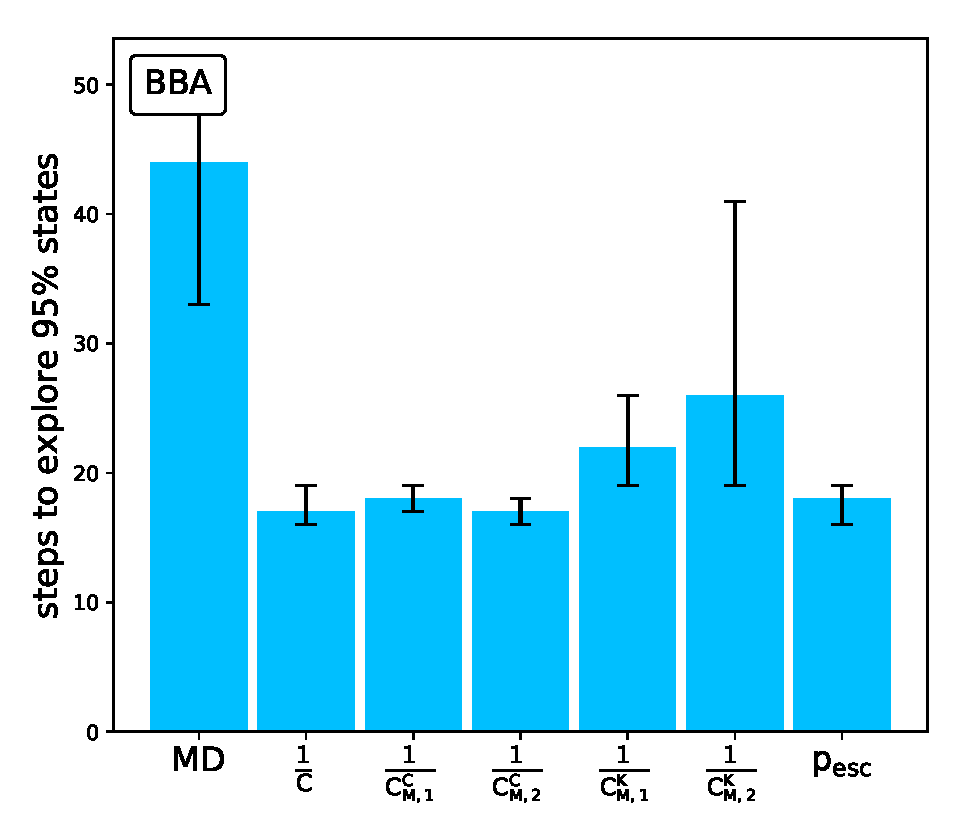
\includegraphics[width=0.9\textwidth]{figures/1FME_7_steps10000_nparallel100_explore.eps}
    %%\caption{WW Domain}    
  \end{subfigure}
  \begin{subfigure}[t]{0.5\textwidth}
    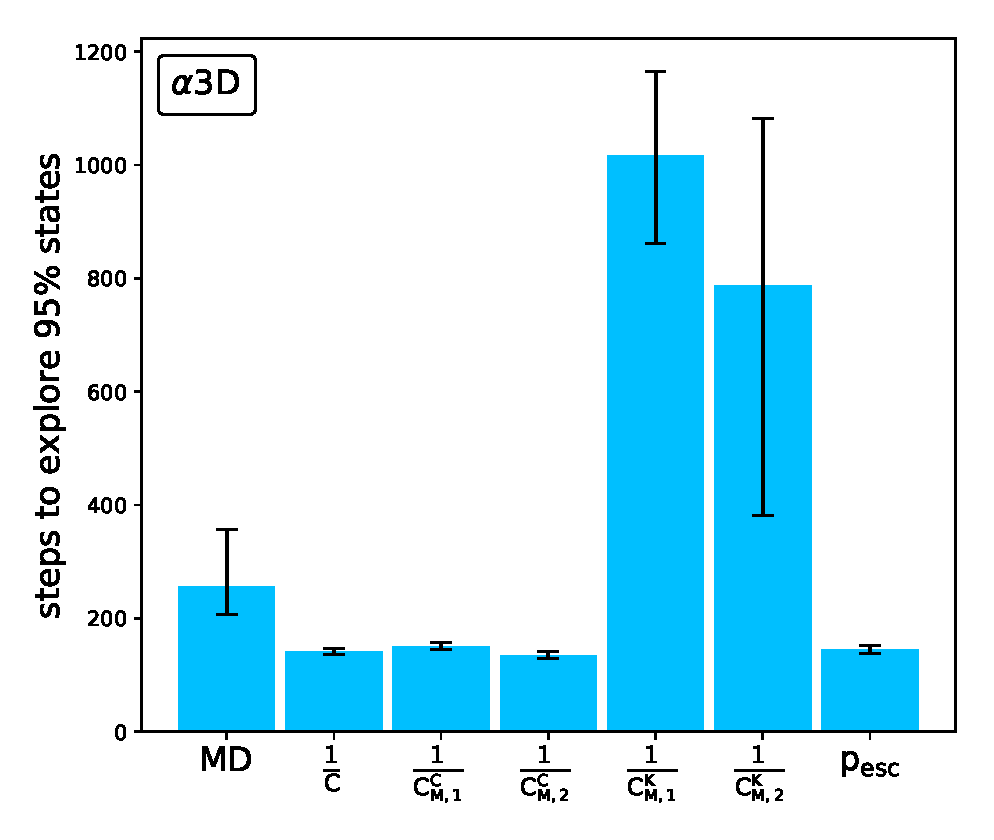
\includegraphics[width=0.9\textwidth]{figures/A3D_7_steps10000_nparallel100_explore.eps}
    %%\caption{$\lambda$-repressor}    
  \end{subfigure}
  %%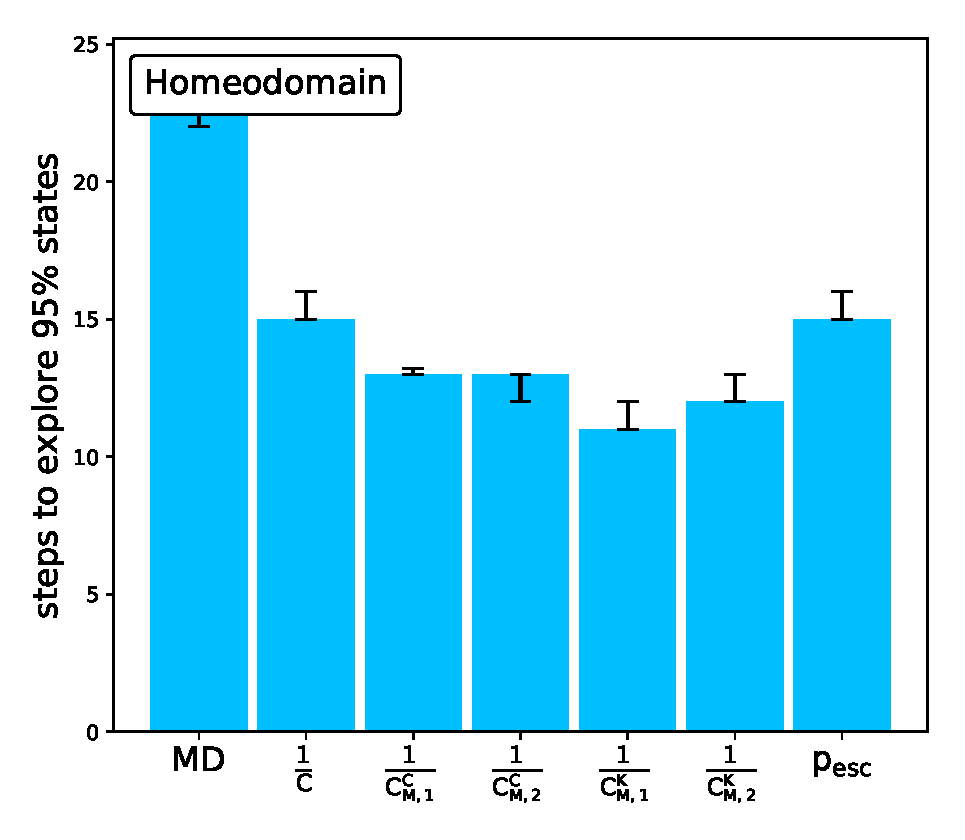
\includegraphics[width=\textwidth]{figures/UVF_7_steps10000_nparallel100_explore.eps}
  \caption{Comparison of the number of steps required to explore 95\% of the
  configurational space for different adaptive sampling strategies for three
  different protein models, by using 100 parallel trajectories. The 20\% and
  80\% percentiles are shown as the error bars.
  The results of the t-test between MD and the
  individual strategies for the different proteins are reported in the Supplementary material.}
  \label{fig:Time_explore}
\end{figure}

Figure~\ref{fig:Time_explore} shows the average time needed for the different
adaptive sampling strategies to explore 95\% of the microstates constituting the
MSM, by using 100 parallel trajectories, for three different proteins.
In this comparison we exclude the strategies designed to speedup the sampling
of the folding process (such as the native contact based strategies as well as
$t_{opt}$) because they are not designed for the purpose of general exploration.
The comparison shows that, in general, the $1/C$ strategy explores the
configurational space much more efficiently than plain MD. The speedup obtained
by the $1/C$ strategy nears the theoretical maximum obtained by the optimal
exploration strategy, $p_{esc}$. Within the macrostate-based strategies, there
is more variance. The strategies using the regular count matrix $(1/C_M^C)$ outperform
the strategies that correct for non-equilibrium errors, $(1/C_M^K)$. This is
likely because the correction introduces a bias towards the sampling of slow
processes rather than general exploration. The non-equilibrium error in the
count matrix based strategies introduces randomness that helps the sampling of
unexplored microstates. Additionally, for some proteins the optimization of the number of
macrostates based on the kinetic content ($1/C_{M, 2}$) does appear to provide
an advantage over the use of a constant number of macrostates ($1/C_{M, 1}$). 
The use of the kinetic content allows for a more accurate estimation of
macrostate counts, which could help to focus the sampling bias towards regions
that are less densely sampled. 
The patterns shown in Fig.~\ref{fig:Time_explore}
are consistent across all the proteins and across the number of
parallel trajectories used. The corresponding plots for all the proteins can be
found in the Supplementary material.

\subsection{\label{sec:scaling}Scaling}

\begin{figure}[t]
  %%\centering
  \begin{subfigure}[t]{0.5\textwidth}
    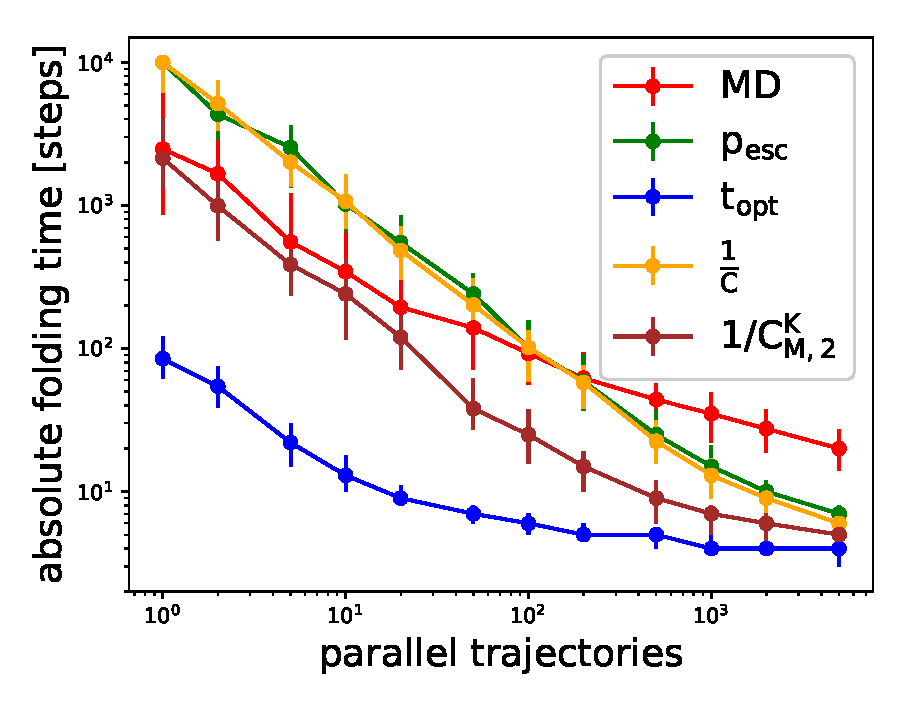
\includegraphics[width=0.9\textwidth]{figures/GTT_6_steps10000_scaling_fold0.eps}    
  \end{subfigure}
  \begin{subfigure}[t]{0.5\textwidth}
    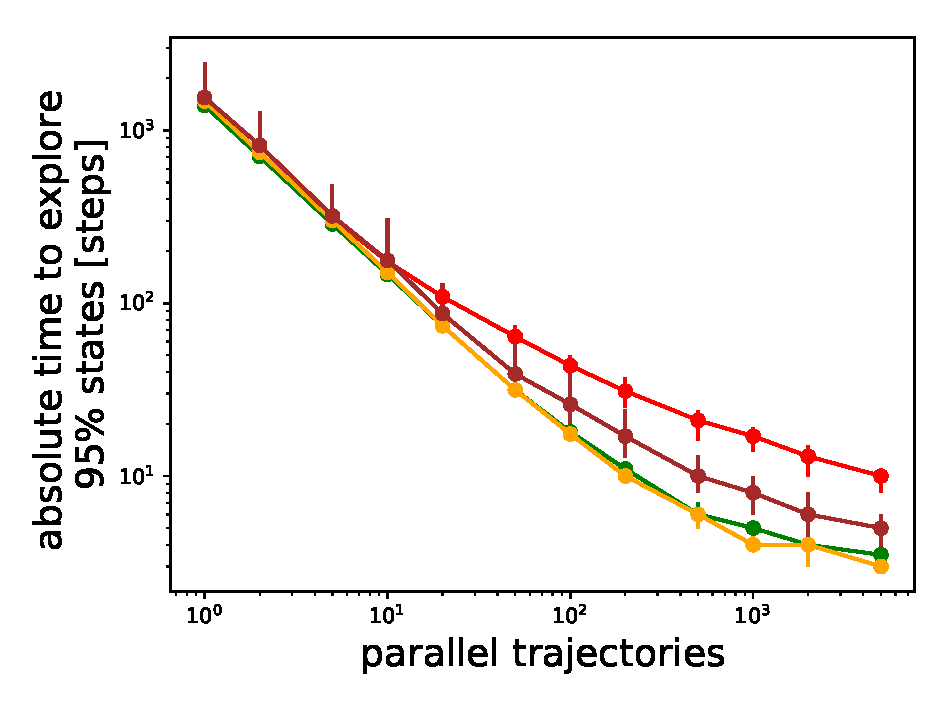
\includegraphics[width=0.9\textwidth]{figures/1FME_6_steps10000_scaling_explore.eps}
    %%\caption{$\lambda$-repressor}    
  \end{subfigure}
  \begin{subfigure}[t]{0.5\textwidth}
    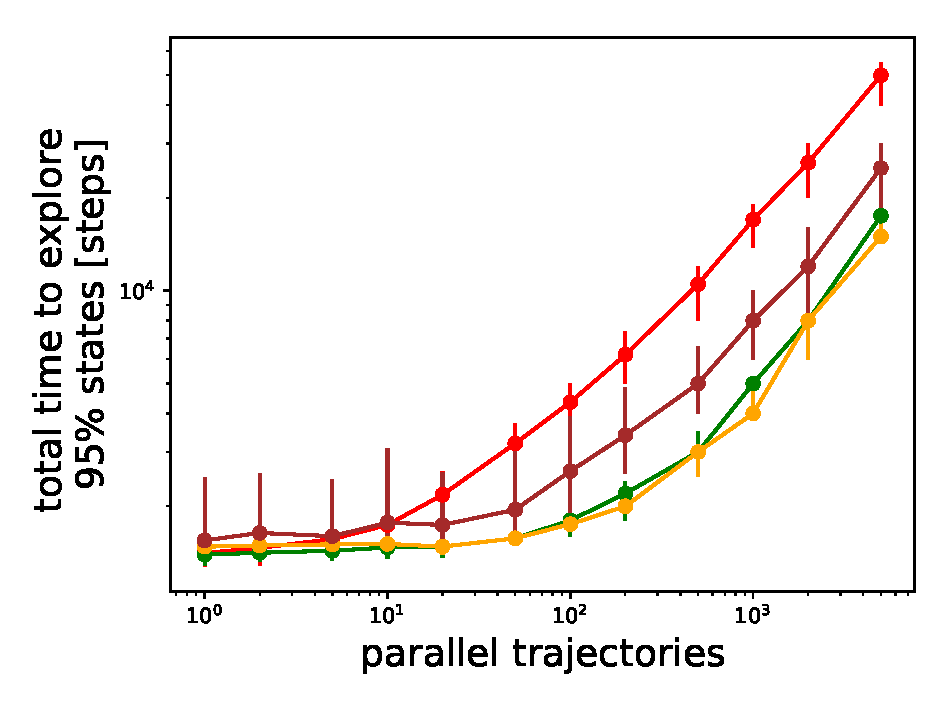
\includegraphics[width=0.9\textwidth]{figures/1FME_6_steps10000_scaling_explore_total.eps}
    %%\caption{$\lambda$-repressor}    
  \end{subfigure}
  \caption{Top: Scaling of the absolute folding time required to fold the
  protein model for the WW Domain for 5 different sampling strategies: plain
  $MD$, $p_{esc}$, $t_{opt}$, $1/C$ and $1/C_{M,2}^K$. Scaling of the
  absolute (middle) or cumulative (bottom) number of steps required to explore
  95\% of all microstates, for the protein  model of BBA, for 3 different
  strategies: plain $MD$, $p_{esc}$, $1/C$ and $1/C_{M,2}^K$.  
  The 20\% and 80\% percentiles are shown as error bars. 
  Similar figures for the other
  protein models are reported in the Supplementary material.}
  \label{fig:scaling}
\end{figure}

Adaptive sampling methods capitalize on the use of many relatively short
parallel trajectories, usually deployed on massively parallel computers (MPC),
to speed up rare events or explore protein conformational spaces. In order to
better understand the limits of scalability of adaptive sampling strategies,
the measured absolute folding time for different parallelization is shown in
Figure \ref{fig:scaling}. The absolute folding time indicates the actual clock
time required to record a folding event for a given protein on MPC with a given
adaptive sampling strategy. The different strategies exhibit good scaling below
a parallelization of around 100 and moderate scalability up to 1000 parallel
trajectories. The scalability differs only slightly between different
strategies, confirming that adaptive sampling generally scales well.
Similar scaling is observed for all protein models. The time to explore 95\% of
microstates in Figure \ref{fig:scaling} scales to a higher parallelization than
the time to fold the protein. In addition to Fig.
\ref{fig:scaling}, scaling plots for the other protein models are
available in the Supplementary material. 

\begin{figure}[!ht]
  %%\centering
  \begin{subfigure}[t]{0.5\textwidth}
    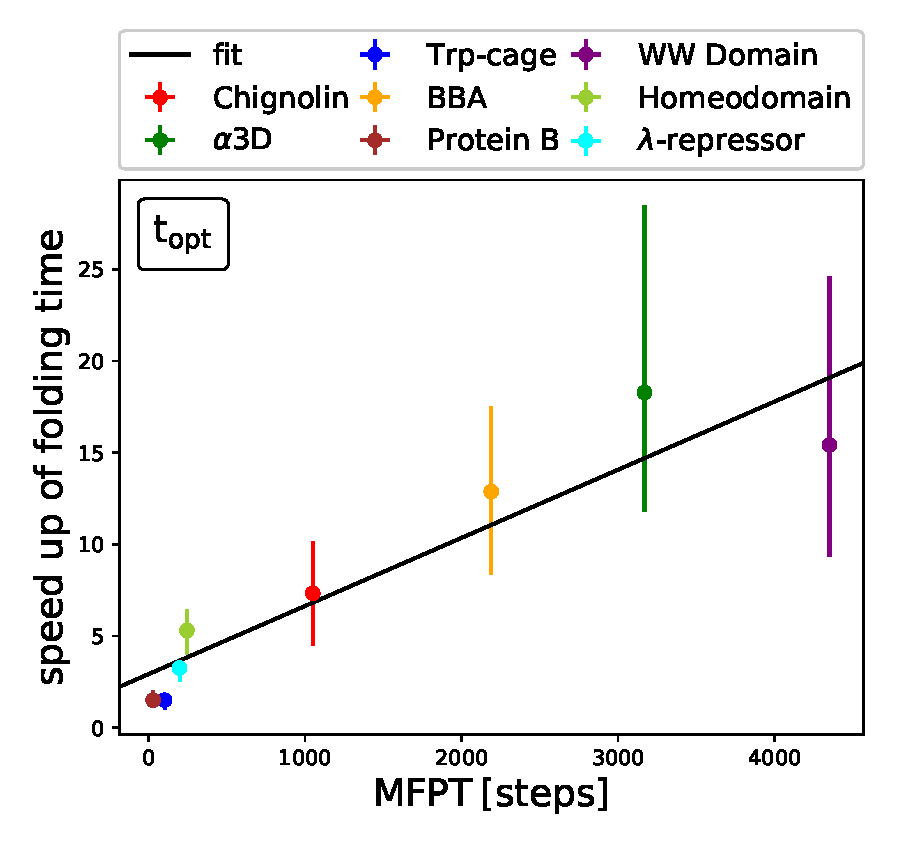
\includegraphics[width=0.9\textwidth]{figures/compare_MD_speed_up_t_opt_6_steps10000_52_0.eps}
    %%\caption{$t_{opt}$}    
  \end{subfigure}
  \begin{subfigure}[t]{0.5\textwidth}
    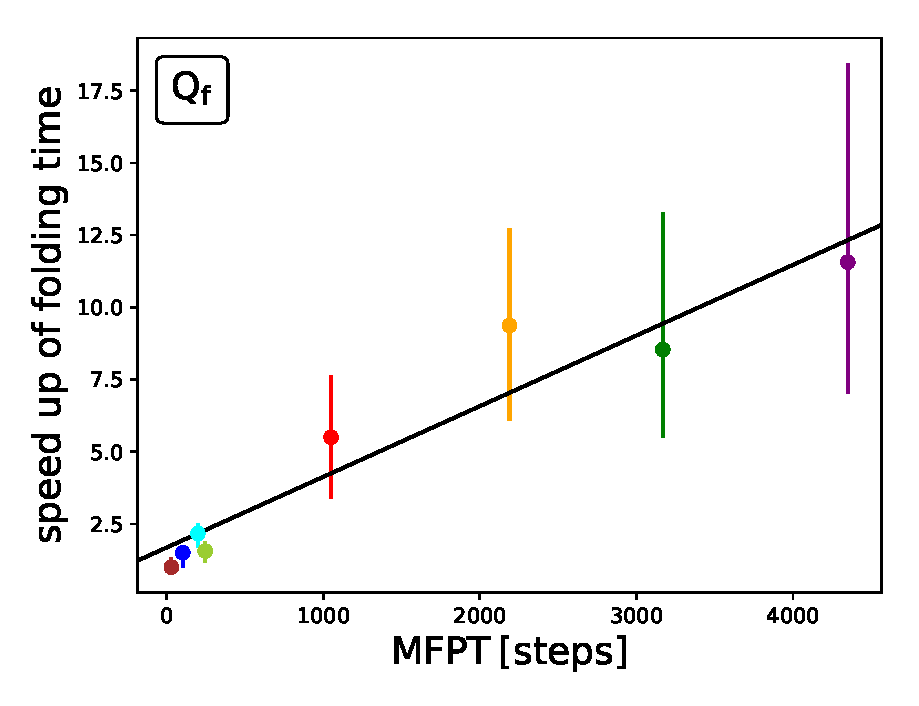
\includegraphics[width=0.9\textwidth]{figures/compare_MD_speed_up_qcore_only_6_steps10000_52.eps}
    %%\caption{$Q_f$}    
  \end{subfigure}
  \begin{subfigure}[t]{0.5\textwidth}
    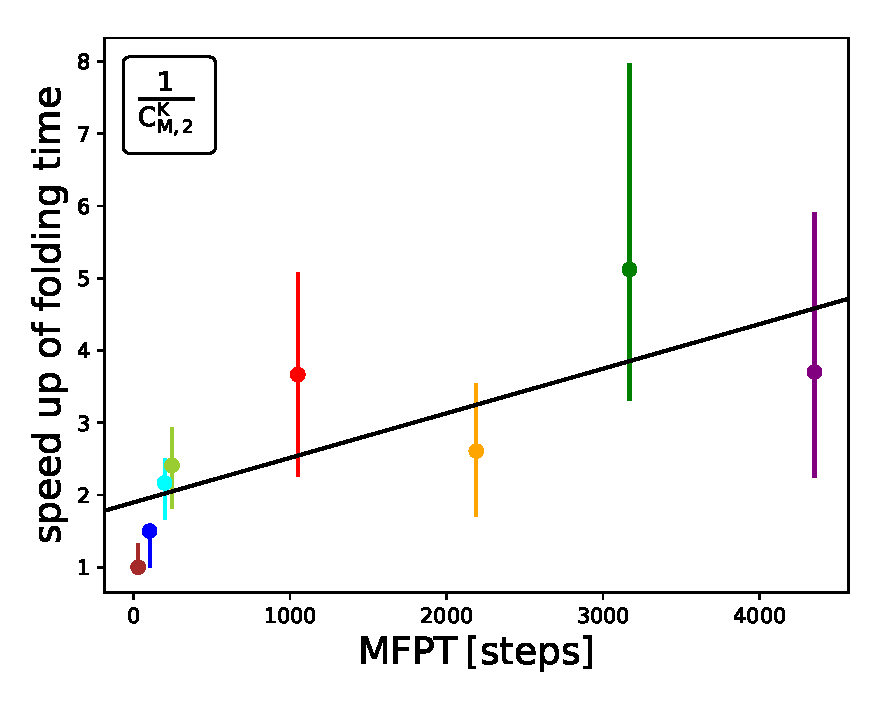
\includegraphics[width=0.9\textwidth]{figures/compare_MD_speed_up_cmacro_kin_cont_50_6_steps10000_52.eps}
    %%\caption{$1/C_{M,2}^K$}
  \end{subfigure}
  \caption{The relationship between the speedup of the folding time with $t_{opt}$, $Q_f$
  or $1/C_{M,2}^K$ vs. mean first passage time for the 8 proteins. Results are reported for a
  parallelization of 100, and the 20\% and 80\% percentiles are shown as error
  bars. The speedup increases with longer MD folding time, the linear fit lines are drawn to guide the eye. The Pearson
  correlation coefficient is for $t_{opt}$ 0.93, for $Q_f$ 0.95 and for
  $1/C_{M,2}^K$ 0.82.}
  \label{fig:compare-MD-speed-cmacro}
\end{figure}


\subsection{\label{sec:compare}Speedup for different proteins}

The speedup in simulating the folding process achieved by using adaptive
sampling in Figure~\ref{fig:Time_fold} varies for different proteins as each
protein has different dynamic properties. In order to better understand the
factors determining the speedup reachable with adaptive sampling strategies, we
compare different properties over the different protein models.

Figure \ref{fig:compare-MD-speed-cmacro} shows that, despite the small sample size
and large error bars, there is a significant correlation between
the theoretical maximum speedup in folding reachable with adaptive sampling
($t_{opt}$) and the folding time of a protein model (as measured by the mean first passage time).
Similar correlations appear for the speedup achieved by using an adaptive
sampling strategy based on the number of macrostates explored upon correction
for non-equilibrium effect ($1/C_{M, 2}$), and also when a reaction coordinate
is used to guide the adaptive sampling ($Q_f$).
That is, for slower folding proteins the efficiency of adaptive sampling
strategies in accelerating the folding rare event increases. This result is
very encouraging for the use of adaptive sampling strategies to sample slow
processes, as adaptive sampling seems to perform better as the processes become
slower. The large error bars are caused by the stochastic nature of the
trajectories. 
No significant correlation is observed between the speedup achieved in folding
and additional properties such as the size of the protein (Figures in Supplementary material).


\section{\label{sec:conclusion}Conclusion}

We have presented a systematic analysis of the performance of different
adaptive sampling strategies by using as test systems 8 different discrete
protein models defined from long all-atom MD simulations.
We have shown that different adaptive sampling strategies are optimal for
different goals. In particular, if the goal of adaptive sampling is to speedup
the simulation of a rare event (such as a protein folding process), it is
important to be able to analyze the explored space on-the-fly and extract a few
metastable states from which new simulations can be restarted. In the data
analysis, it is also important to take into account the effect of
non-equilibrium sampling. Indeed, our results show that a more accurate
estimation of an equilibrium MSM from short non-equilibrium simulations, that
can be obtained by using corrections based on the estimation of the Koopman
operator \cite{koopmanold, koopman2,koopman3,koopman4,  wu2017variational,
Nueske2017}, significantly improve the adaptive sampling of a
protein folding process with respect to a simple estimation of the MSM directly
from non-equilibrium transition counts.

Different considerations are important if the goal of adaptive sampling is to
speedup the exploration of any new regions of the configurational space of a
protein system. In this case, it appears that the most efficient adaptive
sampling strategy is based on the on-the-fly identification of a large number
of kinetic microstates from the simulations already performed, and corrections
for non-equilibrium effects do not appear relevant.
These results suggest that different strategies could be used in different
stages of investigation of a given biophysical process. For instance, the
sampling of rare events could be optimized in a first stage to discover slow
processes in a new system of interest, followed by a second stage where the
different metastable regions in the conformational space can be better sampled
by an adaptive sampling strategy optimized for fast exploration.

We have compared the speedup achieved with the different adaptive sampling
strategies with theoretically optimal benchmark strategies for these two
different goals, $p_{esc}$ and $t_{opt}$, respectively.  The gap between the
speedup of the theoretically optimal strategies and the best performers among
the strategies presented suggest that there could be even faster 
adaptive sampling methods and further investigation in this direction is underway.

We have also shown that, if there is a priori knowledge about the process
under investigation, as for example a reaction coordinate, then adaptive
sampling strategies for the sampling of rare events can be designed to achieve
a speedup close to the theoretical maximum benchmark. In particular, we have
shown that using the number of native (and non-native) contacts to guide the sampling, a
significant improvement in the adaptive sampling of the folding process is
obtained with respect to adaptive sampling strategies that do not use a priori
knowledge of the system.

The adaptive sampling strategies reported here scale well with parallelization
up to about 1000 for the investigated systems.  This result generalizes what
was reported in \cite{bowman2010enhanced} for different proteins. 

Although the best performing adaptive sampling strategies presented here show a
robust speedup over plain MD over a number of different protein models, a significant
variation in performance is observed. Interestingly, the
speedup obtained with the best performing adaptive sampling strategies for
the sampling of the folding process for different protein models correlates
with the folding time as measured with plain MD simulations.
Instead, the size of the proteins or the height of the folding free energy
barrier for the different proteins do not appear to be a strong determinant for
the speedup obtainable by adaptive sampling.
A cautious extrapolation of the correlation between the adaptive sampling
performance and the timescale of the folding rare event encourages the
application of these methods for the characterization of slower processes,
beyond the fast-folding proteins considered here. Due to the limited
number of investigated proteins and the discrete nature of the models used,
the upper limit of the speedup achievable with adaptive sampling methods
for the sampling of rare events cannot be directly estimated from what is
presented here.

\section{\label{sec:res}Results and Discussion}